\documentclass[10pt,a4paper,twocolumn]{article}
\usepackage[utf8]{inputenc}
\usepackage{amsmath}
\usepackage{amsfonts}
\usepackage{amssymb}
\usepackage{graphicx}
\usepackage{url}
\usepackage{subcaption}
\usepackage[left=3cm,right=3cm,top=3cm,bottom=2cm]{geometry}
\author{Micky Faas}
\title{Open-Air Acoustic Delay-line Memory using a Micro-controller}

\begin{document}
\maketitle

\section{Introduction}
Acoustic delay line memory\footnote{From the 1960s and onwards, also other forms of delay line memory (e.g. electromagnetic) were explored and used. In this article whenever \emph{delay line memory} is written, actually the early \emph{acoustic} variant is referred to.} was an early form of computer memory commonly used in the 1940s and 1950s by (mainly, but not exclusively) the EDVAC and later UNIVAC. It was originally invented by John Eckert during his work on the ENIAC, one of the first programmable electronic computers. The paper written by Auerbach et al.\cite{auerbach} provides an overview of the state-of-the-art at that time and has also served as a source of inspriration for the project described in this article.

Eckert's delay line memory is in some ways a generalization of the mercury delay lines developed for radar during WWII. Its operation is based on the concept of generating pressure waves in some medium (in Eckert's case, mercury) using a (transmitting) transducer. The pressure wave is detected by another (receiving) transducer at the other end of the medium. The detected signal is then reshaped, amplified and fed back into the transmitting transducer, resulting in an infinite cycle. For the time it takes the pressure wave to reach the other side of the medium, it is considered to be `stored' inside the medium. Although this time is relatively short (given by the speed of sound in the particular medium), multiple pulses can be stored in serial providing a multi-bit memory - provided that the wave length is short enough and the supporting circuitry is sufficiently fast. Knowing the exact length of the medium one can calculate the exact number of pulses that fit sequentially (essentially the size of the stored memory in bits). A precise clock circuit is used to count the pulses in each refresh cycle allowing a specific bit to be accessed (either read or toggled). 

In this article a (lossy) reconstruction is discussed of the said memory, with the one exception that air is used as medium instead of mercury. The biggest issue with the delay line memory technology - and prime reason for its rapid abandonment - is the fact maintaining a stable medium is very hard. Environmental conditions such as temperature and acoustic noise greatly influence the performance and must therefore be controlled tightly. As this experiment serves a proof-of-concept purpose only, we have no requirements for its actual stability or longevity. 

\subsection{Related work}
While this article is loosely based on the work by Auerbach et al.\cite{auerbach}, there is not really any contemporary scientific related work. Worth of mention is, however, the work of Joseph Allen\cite{allen} who made an 4-bit air-medium delay line memory using only discrete electronics. This is probably the first ever demonstration that an air-medium delay line memory would actually work. The experiment was repeated by Stephen Cass\cite{cass} in the same year with roughly the same components. Both projects have served as a source of inspiration.

\subsection{Concept}
For the project described in this article a micro-controller was used rather than discrete components. This approach has both advantages and disadvantages. The power of a modern micro-controller allows for interesting methods that are hard or impossible to realise using analogue electronics. For example, we will later describe the use of Fourier transform in an attempt to implement bit parallel operation. Other advantages include shorter development time and most prominently, a direct interface with the digital domain. The biggest disadvantage is that even a very fast micro-controller cannot rival the near-instantaneous operation of analogue components. The conversion to the digital domain alone requires several discrete time steps (sample-and-hold ADC). As operations cannot be executed in parallel, a certain scheduling needs to be implemented. A delay line memory is inherently parallel and timing critical, so this scheduling must be an order of magnitude faster than the shortest pulse and must be real-time. Fortunately a modern micro-controller can meet the above requirements.

The project described here is built using only off-the-shelf components in order to make the prototype as simple as possible and easily replicable. Furthermore it is part of a larger project to demonstrate the abstract concept of `memory' and make it more tangible. With an air-medium acoustic delay line memory, one could actually `experience memory' by occupying the same space as well as interact (distort) the medium by a mere presence. This is, of course, of an artistic  importance rather than a scientific one.

\section{Acoustic Delay Line Memory}
Apart from supporting circuitry, a delay line memory consists of roughly two components: (1) a transducer- and medium assembly and (2) a control and logic circuitry. Component (1) furthermore consists of an analog amplifier and transmitter, the \emph{column} containing the medium and the receiver transducer and a \emph{detector} circuit. The detector amplifies the signal from the receiving end and distinguishes between the presence (1) or absence (0) of a pulse. In component (2) the waveform is \emph{reshaped} before it is fed back to the transmitting end. As analog signals inevitably decay when repeatedly fed into this feedback-loop, it must be somehow reconstructed. As described in \cite{auerbach}, it is possible to do this using some sort of \emph{gating}. By using a clock circuit to give a pulse at the exact same rate that pulses appear at the detector, a simple AND-gate can be used to inject the clock pulse at the transmitting end each time a pulse co-occurs at the receiving end. This ensures a stable feedback loop that does not degrade over time. Lastly, the control and logic part contains the necessary logic to access the requested bit. Obviously, the access time will be at most one complete cycle time and the access-logic must synchronize with the clock to wait for the requested bit to appear.

In the micro-controller approach the second component is realised completely in software by constructing something very much like a real-time digital signal processor (DSP). In the case of air, the assembly is replaced by a simple speaker and amplifier and a microphone on the receiving end. Thus this part is completely in the analogue domain and means that a conversion forth and back must take place before the DSP can use the signal. Figure \ref{fig:dsp} gives an abstract schematic of how the DSP is organized. It connects to the analogue part using a digital-to-analogue converter (DAC, to transmitter) and an analogue-to-digital converter (ADC, to receiver). Additionally it uses a serial interface to allow some external device to read and modify the memory. The serial device accepts simple commands in the spirit of `toggle the $n$-th bit'.  The rest of the DSP's components will be elaborated on in the coming subsections.

\begin{figure}
\centering
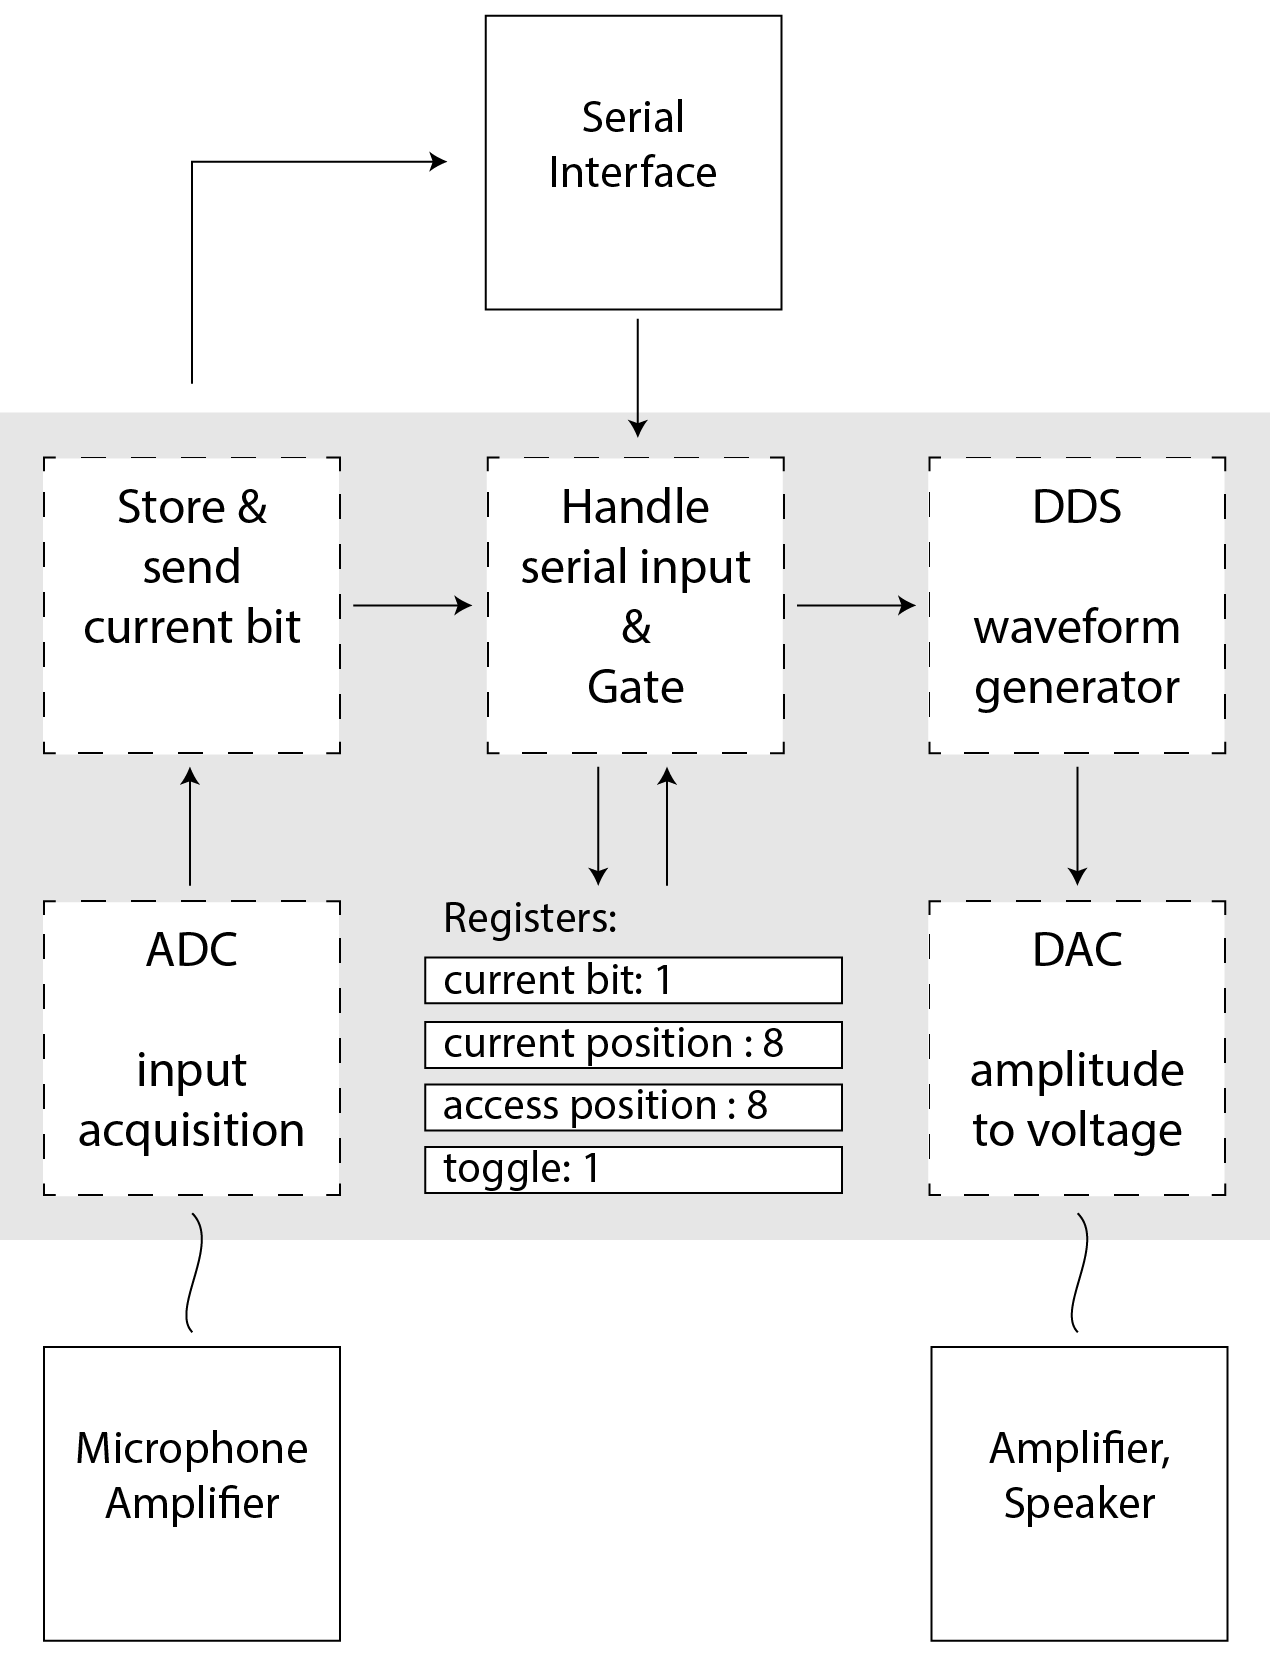
\includegraphics[width=\columnwidth]{delay line dsp-01.png} 
\caption{Block diagram of the signal processing}
\label{fig:dsp}
\end{figure}

\subsection{Bit Serial Operation}\label{bitserial}
We call the delay line memory described in \cite{auerbach} a \emph{bit serial operation}. It is defined as a string of $n$ bits of which currently $n-1$ occupy the delay line. All bits are send sequentially in their original order - this is one \emph{cycle}. The speed of which the string of $n$ bits propagates through the system is the \emph{cycle rate} and is defined by the length of the medium, the speed of sound in that medium at the current temperature and the length of one pulse (thus the frequency of the waveform). In the ideal case this waveform would closely resemble a square wave that has square-shaped pulses exactly at the set bits and zero amplitude at the zero bits. 

In reality, however, such a square wave is composed of a finite number of sinusoids of multiple frequencies (see Figure \ref{fig:squarefourier}) which in turn propagate through the medium at different speeds. Added to this are phase-shifted copies of the original signal caused by reflections off the walls of the medium. The result is a distorted signal that can be described as a \emph{wave packet}. The exact physics behind this problem are beyond the scope of this article, but the consequence is that eventually the \emph{envelope} around the wave is measured at the detector (see Figure \ref{fig:envelope}). The main issue with this is that different pulses will start to overlap as the envelope is larger than the original ideal pulse. In \cite{auerbach} an elegant (analogue) solution is found for this problem, but in this article we utilize the benefits given to us by the digital domain.

There are a number of measures that can be employed in order to create the most stable signal at the detector, however, all come at an additional cost. We can reduce the amplitude (voltage swing) which somewhat reduces the `overhang' of the envelope but also reduces the signal-to-noise ratio. Furthermore the duty-cycle can be reduced, essentially creating more `silence' in between pulses. This effectively increases the frequency of the system, generating other (unwanted) harmonics while requiring faster switching of the output rail. Lastly we can adjust the window in which input samples are collected at the detector. This means that distortion at the boundaries of the pulse are ignored. However, less samples provide less stability and smaller windows (and duty cycles) require stricter timing and better calibrated distance.  Figure \ref{fig:detect} summarizes some of the mentioned `tweaking' possibilities. In the actual implementation these measures are parametrized and set through the serial interface such that they can be used to calibrate a live system.

\begin{figure}[t!]
    \centering
    \begin{subfigure}[t]{\columnwidth}
        \centering
        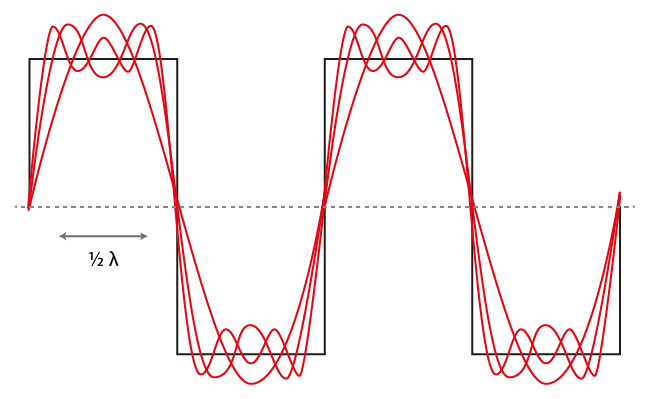
\includegraphics[width=\columnwidth]{squarewave-01.png} 
        \caption{Square wave and its first three Fourier components}
        \label{fig:squarefourier}
    \end{subfigure}%

    \begin{subfigure}[t]{\columnwidth}
        \centering
        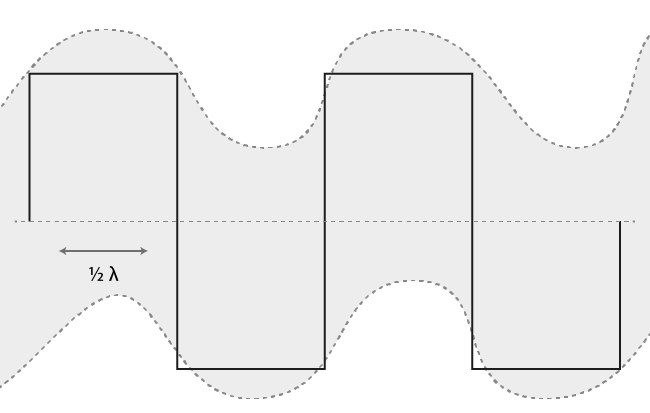
\includegraphics[width=\columnwidth]{squarewave-02.png} 
        \caption{Example of a detected envelope vs. the original waveform}
        \label{fig:envelope}
    \end{subfigure}
    
    \begin{subfigure}[t]{\columnwidth}
        \centering
        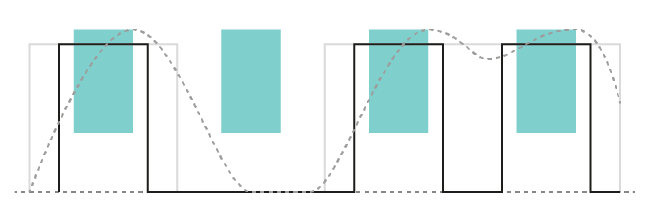
\includegraphics[width=\columnwidth]{squarewave-03.png} 
        \caption{Alleviating detection noise by (1) reducing amplitude and duty-cycle and (2) narrowing detection window (shaded boxes)}
        \label{fig:detect}
    \end{subfigure}
    \caption{Distortion of ideal square wave }
\end{figure}

\subsection{Bit Parallel Operation}
As described in \ref{bitserial}, an attempt to inject a perfect square wave into the medium actually results in a composition of sinusoids. Moreover, a square wave with a 50\% duty-cycle of length $\lambda$ produces exactly the following well-known Fourier series:
$$
f(x) = \frac{4}{\pi} \sum^{\infty}_{n=1,3,5,\dots} \frac{1}{n} \mathrm{sin} \Big ( \frac{n \pi x}{\lambda} \Big )
$$
Now the concept of \emph{bit parallel operation} is to generate the constituent sinusoids of the original square wave up to a finite number. The `depth' of the memory cycle is realised in the same manner as with the serial operation, however, by turning the individual sinusoids on/off \emph{per pulse} multiple bits can be stored on each pulse. This method essentially transforms the delay line into a two-dimensional array of bits, in theory allowing for a much larger memory size.

In order to implement a bit parallel operation the constituent sinusoids must be generated at the transmitting end. Furthermore, the receiving end has to perform Fourier transform on the incoming wave to distinguish between the individual frequencies. Fortunately this is possible in the digital domain, but it also requires vastly more computational power than a simple square wave would.

\subsection{Direct Digital Synthesis}\label{dds}
Direct Digital Synthesis (DDS)\cite{dds} is a method of generating parametric waveforms of multiple frequencies. It is implemented completely in software as opposed to other methods such as discrete hardware oscillators or dedicated waveform generators. The most prominent advantages is that no additional hardware is required and the software solution makes it very flexible. The number of waveforms is, however, limited by the resolution of the DAC and the precision of the calculations. We use DDS in the bit parallel operation to generate the first few constituent sinusoids of the ideal square wave.

Because estimating functions like $sin(x)$ is computationally costly, a DDS system contains a buffer that holds pre-calculated amplitudes for the type of waveform it is to generate. This buffer is sampled at constant intervals at some timer interrupt. The frequency of these samplings is the \emph{reference clock} $F_{clk}$. The exact sample that is to be taken from the buffer is stored, per output wave, in a \emph{phase accumulator}. This is a register of $N$ bits that is being incremented before  every sampling. The amount with which the phase accumulator is incremented is a constant called the \emph{tuning word} M; it defines the relation between the reference clock $F_{clk}$ and the desired output frequency $F$ and is defined by:
$$
M = \frac{2^NF}{F_{clk}}
$$

When multiple waveforms of different frequencies are desired, multiple phase accumulators with their respective tuning words are required. The resulting amplitudes are added after all sampling is complete and are written to the DAC. Obviously, the resolution of the DAC places an upper bound on the number of amplitudes that can be added together. As this system uses only simple additions and lookups in (ROM) memory, it is very efficient and low-cost. 

\section{Implementation}
Both operating modes (serial and parallel) were implemented on an Atmel SAMD21 micro-controller\cite{samd21} and an off-the-shelve microphone amplifier, class-D power amplifier and simple speaker and electret microphone. The SAMD21 is based on the ARM Cortex M0+-architecture and is available on many different prefabricated prototype boards (this particular one was from Arduino). It was chosen mostly for its built-in 10-bit DAC and 12-bit ADC, and its ability to do hardware-accelerated FFT/FHT. Other features include 32-bit arithmetic (which includes floating point), a serial interface (over USB), numerous high-precision timers and 32KB SRAM.

The same setup was used for both operating modes. The SAMD21 was connected through port \texttt{DAC0} to a PAM8403 power amplifier, which in turn was connected to a speaker through a simple RC high-pass filter ($F_0 = 800\mathrm{hz}$). The speaker used was a simple 4 ohm rated dynamic mid-high with a response of 1000-15,000 Hz +/- 3 dB and 88 dB / 1 W sensitivity. Pin PA5 (Arduino A4, could be any ADC pin, really) was used to connect the micro-controller to a MAX4466 microphone amplifier and a simple electrec microphone (multiple were tested and quality varied greatly across different specimen). The SAMD21 was powered from the USB-port (also used to power the amplifiers). The Arduino environment/library was used for the serial connection and for all other functionalities the standard libraries from Atmel were used.

\subsection{Bit Serial Operating Mode}
The serial operating mode is the most simplistic (and successful) version. Its code can be found in the \texttt{delayline\_samd21.ino} file in the repository\cite{repo}. The serial connection is managed in the \texttt{loop()} provided by the Arduino environment. Since this mainloop has a high latency it cannot be used for any time-critical applications. Because the simple nature of the computations, it was decided that all other instructions can be placed in the ADC's interrupt handler (function \texttt{ADC\_Handler()}.

Timing is the most important part of the correct operation of the delay line. Therefore, the ADC is carefully clocked to ensure that samples can be obtained as quickly as possible while allowing enough cycles to process the samples and write to the DAC. Both the ADC clock (\texttt{GCLK\_ADC}) and DAC clock (\texttt{GCLK\_DAC}) are clocked from general clock 0 (\texttt{GCLK0}), which in turn is set to the master clock at 48 Mhz (prescaler 1). \texttt{GCLK\_ADC} is prescaled by 128, giving it an effective clock speed of 375 Khz. The ADC's resolution is set to 8 bit and per the SAMD21 datasheet it takes 5 cycles to sample 8 bits, so the effective sample rate is 75 Khz. By default, the period of the square pulse is set to 8 ADC samples (this is an optional parameter) giving it a principal frequency of 18.75 Khz - just in the audible range\footnote{In reality, due to the irregularly shaped waveform and the less than 50\% duty-cycle, the produced sound is all over the spectrum.}. 

The number above tells us that roughly every 0.053 ms a pulse can be detected. In this time a pulse travels $5.3\cdot10^{-5}\cdot343=0.018\mathrm{m}$ ($v=343\mathrm{ms}^{-1}$, air at 20$^{\circ}$ C). Note that as 0.053 ms gives us the frequency of 18.75 Khz, length of a pulse is also exactly $\frac{343}{18.75\cdot10^3}=0.018\mathrm{m}$. Theoretically, this gives roughly 50 bits per meter of air. If we can increase the frequency of both the sampling and the output waveform, we can increase the amount of storage per meter proportionally (if the hardware permits this, of course).

\subsection{Bit Parallel Operating Mode} 
A bit-parallel mode requires a more complex approach. First of all the individual sinusoids need to be produced using DDS (see \ref{dds}). The DDS uses a 256-element sinusoid in flash ROM and hardware timer \texttt{TC3} is used to increment up to five phase accumulators. By using \texttt{TC5} in 8-bit mode with a prescaler of 8 from the master clock, we obtain a frequency of just over 23 Khz (giving a maximum sine frequency of 11.8 Khz by Nyquist). An additional register of 5 bits can be used to control whether each sinusoid is enabled or not.

On the receiving end we prepare the ADC in the same way as in the previous section, albeit a little slower (prescaler 256, 10-bit mode giving a sample rate of 31.25 Khz). This extra time allows for a simple FFT analysis of the incoming samples. The hardware (r)FFT instructions can be accessed through the CMSIS-DSP library that comes with the Cortex M series of micro-controllers\cite{cmsis}. Despite the hardware acceleration, FFT proved not to be a particularly strong suit of the SAMD21 though. In the end the bare minimal rFFT was used on the \texttt{q15} datatype (signed 16-bit integer), with a Hamming window of 32 samples and no overlap. In theory, this means an FFT-analysis could be performed every 1.02 ms. 

A detection rate of 1.02 ms tells us that the different `frames' of parallel bits should be physically apart by $343\mathrm{ms}^{-1}\cdot1.02\cdot10^{-3}\mathrm{s}=0.35\mathrm{m}$. The wave lengths of the individual sinusoids should obviously still be an order of magnitude smaller that this figure. Given that using a window size of 32 samples we can distinguish between 5 different frequencies (this is an empirical number), we can store roughly 14 bits per meter. Unfortunately this is (at least theoretically) inferior to the much simpler bit serial operating mode.

\section{Discussion}
Only preliminary experiments have been conducted so far, showing that a practical setup is far less forgiving than what the theoretical analysis predicts. Factors such as room acoustics, latency from the micro-controller and analogue losses from the components (mainly the microphone and its amplifier) make that less-than-ideal results are obtained.
During tests of the bit-serial program a stable delay line of 5 bits in roughly 3 meters could be achieved, a factor 30 worse than predicted. For the bit-parallel program an array of $1 \times 5$ bits could be achieved (frames of 5-bit, cycles of 1 deep). While this is not even technically a delay line yet, it shows that the method using DDS and FFT can be effective and will probably work on a faster micro-controller.
While the results can hopefully be improved by using higher quality analogue components, a faster micro-controller and better controlled room conditions, experiments also showed another issue. Although this problem is subjective in nature, the sound levels required to obtain a sufficient signal-to-noise ratio in the receiver were \emph{unbearably loud}. In conjunction with the harmonics produced by the square waves it is very uncomfortable for a person to be in the same room with the delay line memory. While scientifically irrelevant, this greatly impairs the idea of using the project in a demo or installation.

A possible remedy to this problem is the use of supersonic frequencies, outside the audible hearing range. Because of the shorter wave lengths this also means that better storage figures could be achieved. Although even better equipment would required to detect shorter pulses, it is nonetheless an interesting proposition that warrants further experimentation.  


\begin{thebibliography}{}

\bibitem{auerbach}
I. L. Auerbach, J. P. Eckert, R. F. Shaw and C. B. Sheppard, ``Mercury Delay Line Memory Using a Pulse Rate of Several Megacycles,'' in Proceedings of the IRE, vol. 37, no. 8, pp. 855-861, Aug. 1949.

\bibitem{allen}
J. Allen, ``Acoustic delay line memory''. \url{http://jhallenworld.blogspot.nl/2014/01/acoustic-delay-line-memory.html}. 2014.

\bibitem{cass}
S. Cass, ``Build a Delay-Line Memory Out of (Mostly) Thin Air''. \url{https://spectrum.ieee.org/geek-life/hands-on/build-a-delayline-memory-out-of-mostly-thin-air}. 2014.

\bibitem{dds}
Analog Devices Inc., ``A Technical Tutorial on Digital Signal Synthesis''. 1999.
\url{https://ieee.li/pdf/essay/dds.pdf}

\bibitem{samd21}
Atmel/Microship.com, ATSAMD21G18 series micro-controller.
\url{https://www.microchip.com/wwwproducts/en/ATSAMD21G18}

\bibitem{repo}
M.E. Faas, ``Open-Air Acoustic Delay-line Memory using SAMD21''. \url{https://github.com/mickymuis/delayline}

\bibitem{cmsis}
ARM ltd., ``Cortex Microcontroller Software Interface Standard''. \url{https://developer.arm.com/embedded/cmsis}

\end{thebibliography}

\end{document}